\chapter{SYSTEM DESIGN}

\section{Requirement Specification}

\subsection{Functional Requirement}

\subsubsection{User Registration and Profile Management}
Users can create accounts, manage profiles, and update preferences such as interests, travel dates, and accessibility requirements.

\subsubsection{Recommendation Generation}
Utilizing recommendation algorithms, the system generates personalized attraction recommendations based on user preferences, location, time constraints, and historical data.

%\subsubsection{Feedback Mechanism}
%Users can provide feedback, ratings, and reviews for recommended attractions, which are used to improve future recommendations.

\subsubsection{Integration with Mapping Services}
Seamless integration with mapping services enables users to navigate to recommended attractions with ease.

\subsubsection{User Interface}
The user interface presents recommendations in an intuitive format, allowing users to view attraction details, ratings, reviews, and real-time updates.

%\subsection{Non-Functional Requirement}

%\subsubsection{Compatibility}
%The system should be compatible with modern web browsers, mobile devices to reach a wide audience.

%\subsubsection{Reliability}
%Ensure high system availability, with minimal downtime and robust error handling mechanisms.

%\subsubsection{Maintainability}
%Design the system with modular components, clear documentation, and version control to facilitate ongoing maintenance and updates.

%\subsubsection{Usability}
%The user interface should be user-friendly, accessible across devices, and provide a seamless experience for tourists of all demographics.

%\subsubsection{Security}
%Implement robust security measures to protect user data, prevent unauthorized access, and ensure data privacy compliance.

%\section{Feasibility Assessment}

%\subsection{Technical Feasibility}
%Evaluate the technical feasibility of implementing the recommendation system, considering factors such as data collection, algorithm complexity, and integration with external services.

%\subsection{Schedule Feasibility}
%Create a project timeline to assess if the project can be completed within the specified timeframe. Identify key milestones, dependencies, and critical path activities to ensure timely completion.

%\subsection{Operational Feasibility}
%Determine the operational feasibility by assessing the impact of the system on existing processes, resource requirements, and organizational readiness for deployment.

%\subsection{Risk Assessment}
%Identify potential risks and challenges that may impact the success of the project. Develop risk mitigation strategies and contingency plans to address unforeseen issues.

\pagebreak

\section{Use Case Diagram}

\begin{figure}[h]
\centering
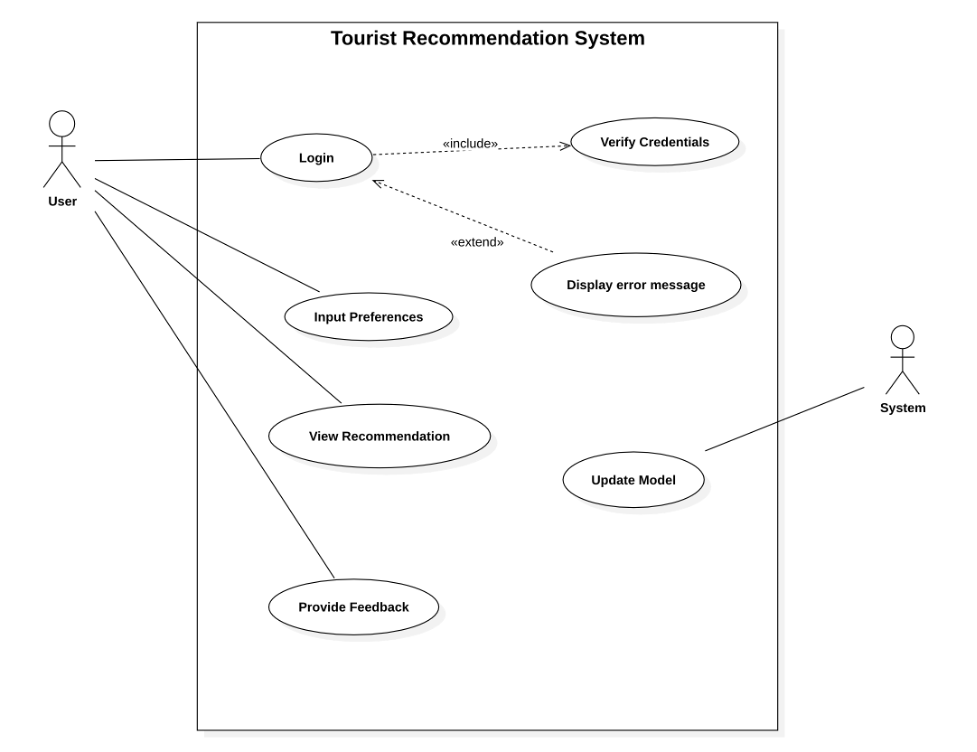
\includegraphics[width=1.0\textwidth]{./img/usecase.png}
\caption{System Use Case Diagram}
\end{figure}

\noindent The user serves as the main actor and can log in, input preferences, view recommendations, and provide feedback. Once logged in, the system verifies credentials and allows the user to submit travel preferences, which are then processed to generate tailored recommendations. These recommendations include places to stay, activities to do, and restaurants to eat at. The user can provide feedback on these suggestions, which the system uses to update its recommendation model. This process ensures that the system continuously improves, with error messages displayed for invalid inputs, enhancing the overall user experience and making future suggestions more accurate and personalized.

%\section{Activity Diagram}

%\section{Class Diagram for System}

%\section{Class Diagram for Data }

%\section{Database Schema}

\newpage

\section{Sequence Diagram}

\begin{figure}[hbt!]
\centering
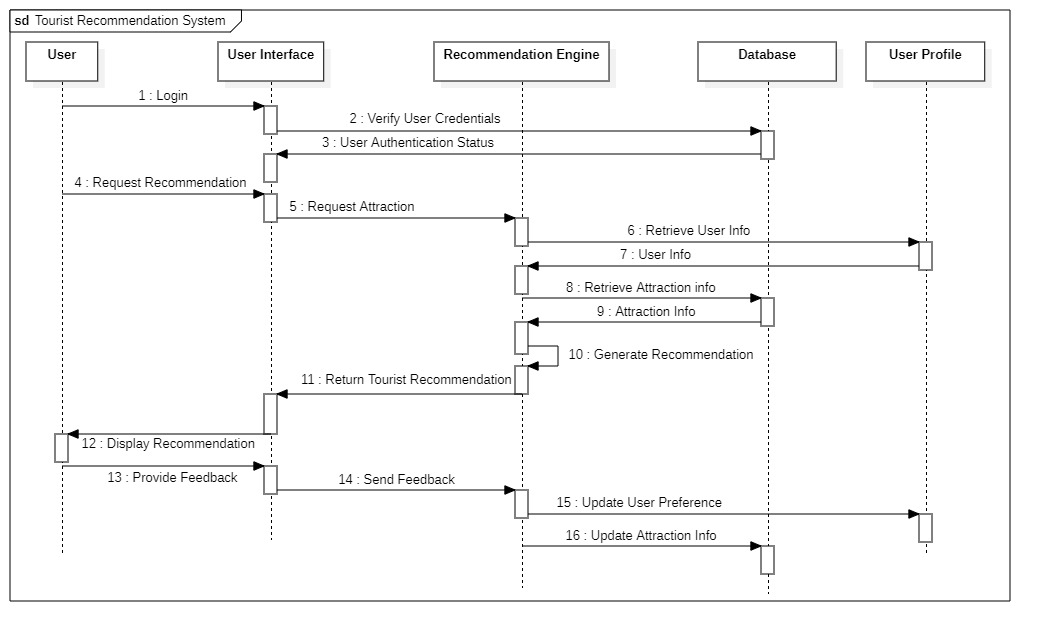
\includegraphics[width=1\textwidth]{./img/SEQ diagram.jpg}
\caption{Sequence Diagram}
\end{figure}

\noindent The sequence diagram illustrates a tourist recommendation system. After logging in and verification, the user requests a recommendation. The system retrieves attraction data, uses the user profile to generate personalized suggestions, and displays them. The user can then view these recommendations and optionally provide feedback. This feedback helps refine the user profile and potentially update attraction information for future recommendations.

%\section{Communication Diagram}

%\section{Data Flow Diagram} 

%\section{Deployment Diagram}

%\textbf{Note: All the diagram is not mandatory..select according to the type of project you are going to do.}
